\documentclass{beamer}
\usepackage[utf8]{inputenc}
\usepackage[T1]{fontenc}
\usepackage[spanish]{babel}
\usepackage{graphicx} 


\usetheme{Madrid}


\includegraphics[width=0.4\textwidth]{images/logouct.png}


\title{Proyecto Restaurante}
\author{
Nicolás Cayumán, Gabriel Gutiérrez y Ailyn Melillán\\[4pt]
\small Programación 2\\
Profesor: Guido Mellado\\
Ayudante: Joaquín Cantero\\
Ingeniería Civil en Informática\\
Universidad Católica de Temuco
}
\date{15/10/2025}

\begin{document}

% Portada
\begin{frame}
  \titlepage
\end{frame}

\begin{frame}{Introducción}
El sector gastronómico enfrenta desafíos de eficiencia operativa y control de recursos.
Los procesos manuales generan:
    \begin{itemize}
            \item Errores humanos
            \item Lentitud
            \item Pérdida de tiempo y dinero
    \end{itemize}
Proponemos una solución digital moderna para automatizar tareas clave del restaurante.
\end{frame}


\begin{frame}{Diagrama}
    \begin{center}
        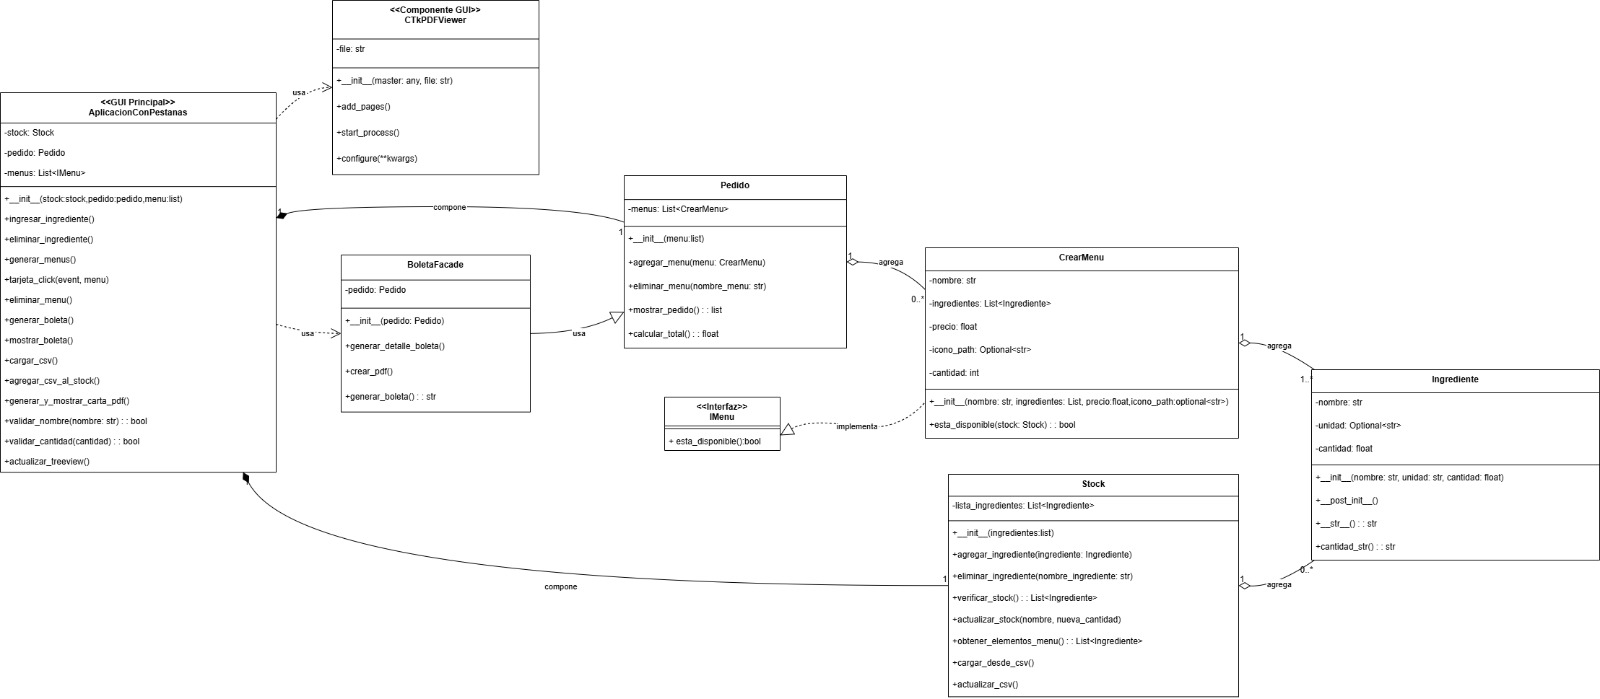
\includegraphics[width=1\textwidth]{images/Diagramaproyecto.png}
    \end{center}
\end{frame}

\begin{frame}{Solución propuesta}
Desarrollamos una aplicación en Python (con CustomTkinter) que digitaliza y automatiza la gestión del restaurante.

Características principales:
\begin{itemize}
    
    \item \textbf{Inventario en tiempo real:} control y carga masiva desde CSV.
    \item \textbf{Toma de pedidos ágil:} verificación automática de stock y descuento inmediato.
    \item \textbf{Generación automática de documentos:} boleta y carta en PDF con visualización integrada.
    \item \textbf{Arquitectura modular:} facilita mantenimiento y escalabilidad.
    \item \textbf{Beneficios:} mayor eficiencia, menos errores, interfaz moderna y documentación digital.
\end{itemize}
\end{frame}


\begin{frame}{Flujo del programa}
El sistema se organiza en tres etapas principales, coordinadas por la clase \textbf{AplicacionConPestanas}.\\
\vfill
\textbf{1. Gestión de Inventario}
\begin{itemize}
    \item Al iniciar, se crea el objeto Stock, que carga los ingredientes desde un archivo CSV.
    \item Carga masiva: el usuario puede subir un CSV con ingredientes para actualizar el inventario.
    \item Gestión manual: se pueden agregar o eliminar ingredientes directamente desde la interfaz.
\end{itemize}
\end{frame}

\begin{frame}{Flujo del programa}
\textbf{2. Ciclo de Venta}
\begin{itemize}
\item En la pestaña Pedido, se muestran los platos del menú.
\item El usuario selecciona un producto → el sistema verifica el stock disponible.
\item Si hay disponibilidad:
    \begin{itemize}
        \item Se descuenta automáticamente la cantidad de ingredientes.
        \item Se actualiza el archivo CSV.
        \item Se agrega el ítem al pedido actual y se recalcula el total.
     \end{itemize}
\end{itemize}
\end{frame}

\begin{frame}{Flujo del programa}
\textbf{3. Documentación}
\begin{itemize}
    \item En la pestaña Carta, se genera el archivo carta.pdf con el menú del restaurante.

    \item En la pestaña Boleta, se crea automáticamente la boleta de venta (boleta.pdf) con subtotal e IVA.

    \item  Ambos PDF se muestran dentro de la aplicación mediante CTkPDFViewer, sin salir de la interfaz.
\end{itemize}
\end{frame}


\begin{frame}{Presentación de la interfaz visual}
    \begin{center}
        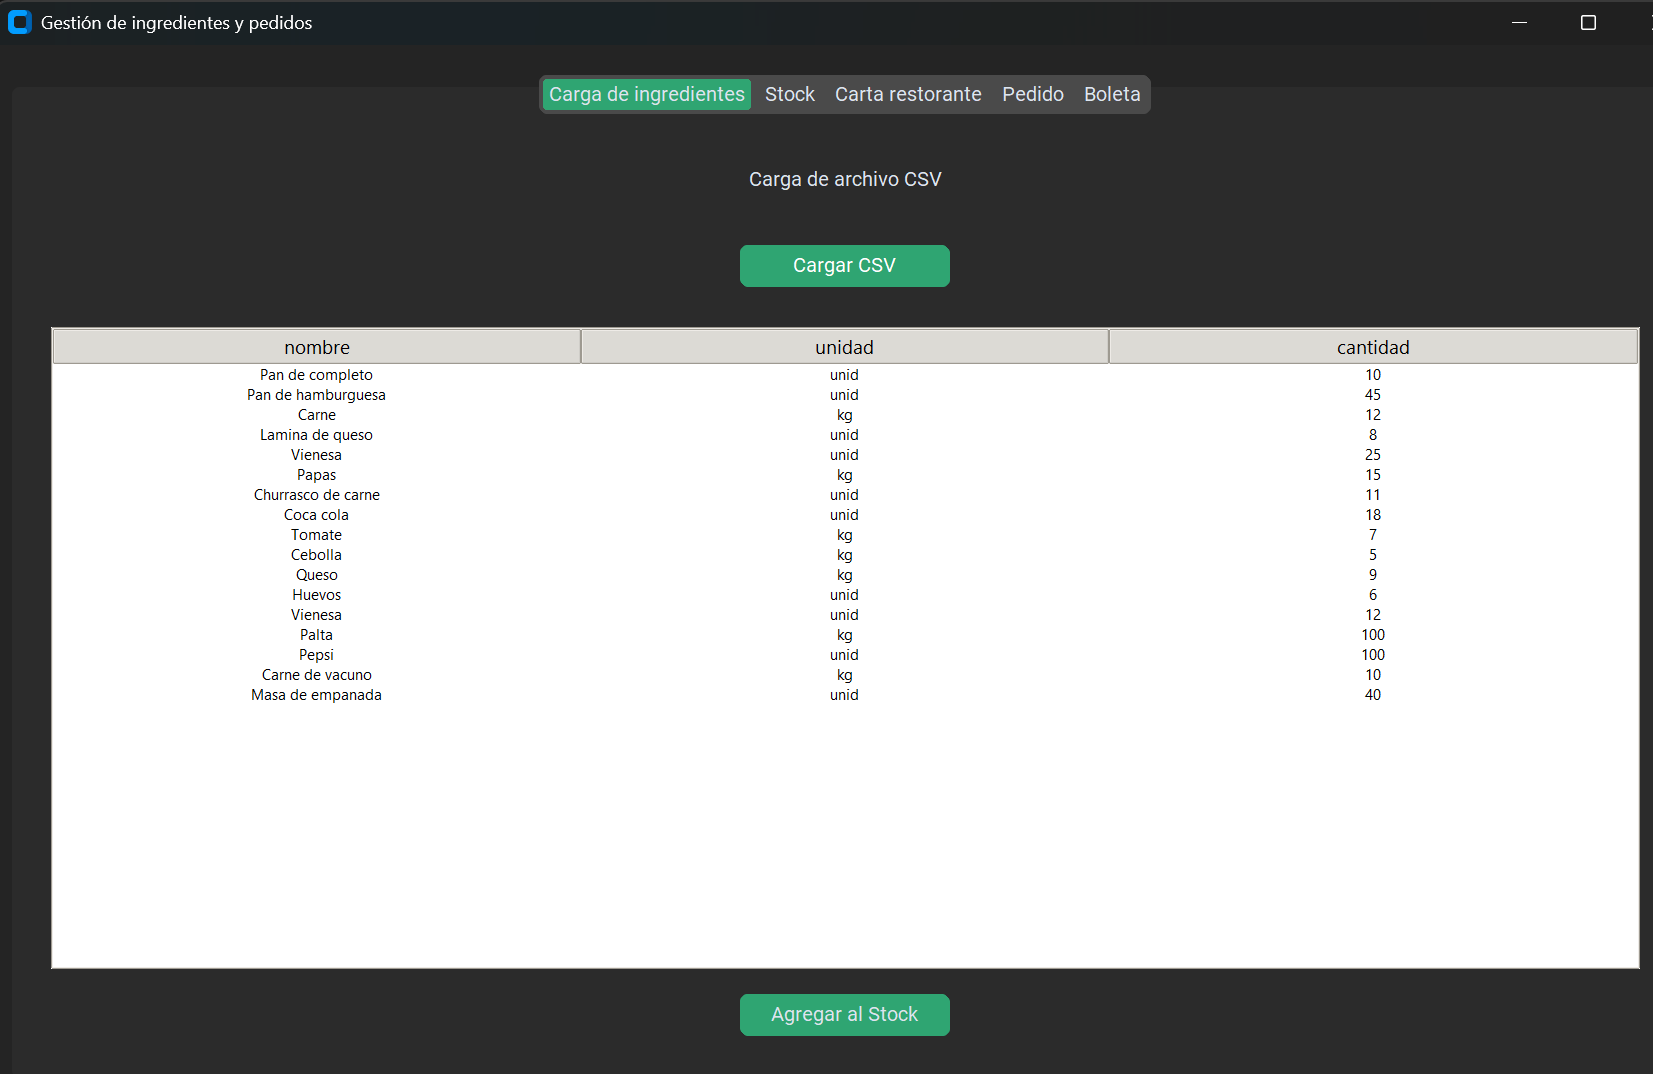
\includegraphics[width=1\textwidth]{images/Interfaz.png}
    \end{center}
\end{frame}


\end{document}